\documentclass{article}
\usepackage{ifplatform}

\ifmacosx
\usepackage[fontset=mac]{ctex}
\fi
\iflinux
\usepackage[fontset=ubuntu]{ctex}
\fi

\usepackage{amsmath}
\usepackage{amssymb}
\usepackage{graphicx}
\usepackage{enumitem}

% http://kuing.orzweb.net/viewthread.php?tid=3004
\newcommand\rsx[1]{\left.{#1}\vphantom{\big|}\right|}

\title{Homework 3 - Image Sentiment Classification}
\author{資工系博士班二年級 D06922023 顏志軒}

\begin{document}

\maketitle

\textbf{Problem 1.} (1\%) 請說明你實作的 CNN model,其模型架構、訓練過程和準確率為何?

我的CNN model使用多層Conv2D+PReLu,以及兩層fully-connected layer,最後是softmax。loss使用cross entropy。詳細model架構如表~\ref{cnn_model}所示。訓練的過程我使用ReduceLROnPlateau,動態的藉由validation set的loss來調整learning。最後得到的準確度為0.6445。

\begin{table}
\caption{CNN model詳細架構}
\label{cnn_model}
\begin{tabular}{c|c|c}
Layer (type) &  Output Shape & Param \#\\
conv2d\_1 (Conv2D) & (None, 44, 44, 64) & 1664\\
p\_re\_lu\_1 (PReLU) & (None, 44, 44, 64) & 123904\\
zero\_padding2d\_1 (ZeroPaddin & (None, 48, 48, 64) & 0\\
max\_pooling2d\_1 (MaxPooling2 & (None, 22, 22, 64) & 0\\
zero\_padding2d\_2 (ZeroPaddin & (None, 24, 24, 64) & 0\\
conv2d\_2 (Conv2D) & (None, 22, 22, 64) & 36928\\
p\_re\_lu\_2 (PReLU) & (None, 22, 22, 64) & 30976\\
zero\_padding2d\_3 (ZeroPaddin & (None, 24, 24, 64) & 0\\
conv2d\_3 (Conv2D) & (None, 22, 22, 64) & 36928\\
p\_re\_lu\_3 (PReLU) & (None, 22, 22, 64) & 30976\\
average\_pooling2d\_1 (Average & (None, 10, 10, 64) & 0\\
zero\_padding2d\_4 (ZeroPaddin & (None, 12, 12, 64) & 0\\
conv2d\_4 (Conv2D) & (None, 10, 10, 128) &  73856\\
p\_re\_lu\_4 (PReLU) & (None, 10, 10, 128) &  12800\\
zero\_padding2d\_5 (ZeroPaddin & (None, 12, 12, 128) &  0\\
conv2d\_5 (Conv2D) & (None, 10, 10, 128) &  147584\\
p\_re\_lu\_5 (PReLU) & (None, 10, 10, 128) &  12800\\
zero\_padding2d\_6 (ZeroPaddin & (None, 12, 12, 128) &  0\\
average\_pooling2d\_2 (Average & (None, 5, 5, 128) &  0\\
flatten\_1 (Flatten) & (None, 3200) & 0\\
dense\_1 (Dense) & (None, 1024) & 3277824\\
p\_re\_lu\_6 (PReLU) & (None, 1024) & 1024\\
dropout\_1 (Dropout) & (None, 1024) & 0\\
dense\_2 (Dense) & (None, 1024) & 1049600\\
p\_re\_lu\_7 (PReLU) & (None, 1024) & 1024\\
dropout\_2 (Dropout) & (None, 1024) & 0\\
dense\_3 (Dense) & (None, 7) &  7175\\
activation\_1 (Activation) & (None, 7) &  0\\
\end{tabular}
\end{table}

\textbf{Problem 2.} (1\%) 承上題,請用與上述 CNN 接近的參數量,實做簡單的 DNN model,其模型架構、訓練過程和準確率為何?試與上題結果做比較,並說明你觀察到了什麼?

我的CNN model中有4845063個參數。我實做如表~\ref{dnn_model}的DNN,有4868871個參數。訓練過程中,調整learning rate的方式與原本的CNN model相同。從第30個epoch開始,就一直維持在training accuracy大約在25\%,而validation accuracy大約在21\%。我判斷這是under fitting,原因可能是DNN無法像CNN藉由圖片的局部特徵來判斷,因此準確度差。

\begin{table}
\caption{DNN model詳細架構}
\label{dnn_model}
\begin{tabular}{c|c|c}
Layer (type)& Output Shape&Param \#\\
dense\_1 (Dense)&(None, 48, 48, 64)&128\\
p\_re\_lu\_1 (PReLU)&(None, 48, 48, 64)&147456\\
dropout\_1 (Dropout)&(None, 48, 48, 64)&0\\
flatten\_1 (Flatten)&(None, 147456)&0\\
dense\_2 (Dense)&(None, 32)&4718624\\
p\_re\_lu\_2 (PReLU)&(None, 32)&32\\
dropout\_2 (Dropout)&(None, 32)&0\\
dense\_3 (Dense)&(None, 64)&2112\\
p\_re\_lu\_3 (PReLU)&(None, 64)&64\\
dropout\_3 (Dropout)&(None, 64)&0\\
dense\_4 (Dense)&(None, 7)& 455\\
activation\_1 (Activation)&(None, 7)& 0\\
\end{tabular}
\end{table}

\textbf{Problem 3.} (1\%) 觀察答錯的圖片中,哪些 class 彼此間容易用混? 並說明你觀察到了什麼? [繪出 confusion matrix 分析]

我用validation set做confusion matrix,結果為:

[ 62   0  14   1   9   8  15]
[  3   4   1   0   0   1   0]
[ 10   0  51   1  17  15   8]
[  0   0   2 136   3   4   8]
[ 13   1  10   3  63   2  21]
[  5   0   6   2   0  72   3]
[  4   0   8   7  17   6  93]

可發現生氣與恐懼、難過與中立容易搞混,可能是這兩類表情彼此較像的緣故。

\textbf{Problem 4.} (1.5\%, each 0.5\%) CNN time/space complexity:\\
For a. b. Given a CNN model as\\
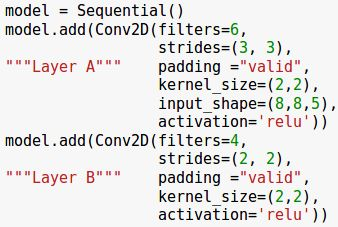
\includegraphics[width=.5\textwidth]{image-000}\\
And for the c. given the parameter as: \\
kernel size = (k, k); \\
channel size = c; \\
input shape of each layer = (n, n); \\
padding = p; \\
strides = (s, s);
\begin{enumerate}[label=(\alph*)]
\item How many parameters are there in each layer(Hint: you may consider whether the number of parameter is related with)\\
Layer A: 6*(2*2)*5 = 120\\
Layer B: Layer A的output有6個channel,故此layer有4*(2*2)*6=96個參數

\item How many multiplications/additions are needed for a forward pass(each layer).\\
Layer A: 一個filter在input feature map上直向和橫向都計算了3次(0-1, 3-4, 6-7),因此總乘法數為6*(2*2)*(3*3)*5 = 1080。總加法數則為6*(3*3)*(2*2*5-1) = 1026。\\
Layer B: Layer A的output為3*3*6,因此Layer B的一個filter在橫向和直向上都只計算了一次(0-1),總乘法數為4*(2*2)*(1*1)*6 = 96,總加法數為4*(1*1)*(2*2*6-1) = 92。

\item  What is the time complexity of convolutional neural networks? (​note: you must use big-O upper bound, and there are l (lower case of L) layer, you can use $C_l$,
$C_{l−1}$ as lth and l-1th layer)

由於乘法的計算成本遠高於加法,因此complexity我只考慮乘法。因為第i層的channel數為i-1層的filter數,因此i層的filter數為i+1層的channel數。l層的總乘法數為:

\begin{equation}
O\left(\sum_{i=1}^{l}\left(\lceil\frac{n_i+2p_i}{s_i}\rceil\right)^2 k_i^2 c_i c_{i+1}\right)
\end{equation}

\end{enumerate}

\textbf{Problem 5.} (1.5\%, each 0.5\%) ​PCA practice: Problem statement: Given 10 samples in 3D space. (1,2,3), (4,8,5), (3,12,9), (1,8,5), (5,14,2), (7,4,1), (9,8,9), (3,8,1), (11,5,6), (10,11,7)
\begin{enumerate}[label=(\alph*)]
\item What are the principal axes?

令這10個點為$\mathbf{x_1}, \mathbf{x_2}, \ldots, \mathbf{x_10}$。這10個點的平均為:

\begin{equation}
\mu = \frac{1}{10}\sum_{n=1}^{10}\mathbf{x_n} = 
\begin{bmatrix}
5.4\\
8\\
4.8
\end{bmatrix}
\end{equation}

其covariance matrix為:
\begin{equation}
\Sigma = \frac{1}{10}\sum_{n=1}^{10} (\mathbf{x_i}-\mathbf{\mu})(\mathbf{x_i}-\mathbf{\mu})^{\mathbf{T}}=
\begin{bmatrix}
12.04 && 0.5 && 3.28\\
0.5 && 12.2 && 2.9\\
3.28 && 2.9 && 8.16\\
\end{bmatrix}
\end{equation}

此矩陣的三個eigenvalue由大到小分別為:$\lambda_1 = 15.30, \lambda_2 = 11.63, \lambda_3 = 5.47$。對應的eigenvector為
\begin{equation}
\mathbf{u_1} = \begin{bmatrix}
-0.62\\
-0.59\\
-0.52\\
\end{bmatrix}, 
\mathbf{u_2} = \begin{bmatrix}
-0.68\\
0.73\\
-0.03\\
\end{bmatrix}, 
\mathbf{u_3} = \begin{bmatrix}
0.40\\
0.34\\
-0.85\\
\end{bmatrix}
\end{equation}

\item Compute the principal components for each sample.

每個點的principal components即為投影到eigenvector的分量,即:
\begin{equation*}
\begin{aligned}
&(-3.36, 0.71, -1.48)\\
&(-9.79, 3.03, 0.04)\\
&(-13.62, 6.53, -2.42)\\
&(-7.94, 5.06, -1.16)\\
&(-12.37, 6.84, 5.02)\\
&(-7.19, -1.84, 3.3)\\
&(-14.96, -0.47, -1.37)\\
&(-7.08, 3.81, 3.05)\\
&(-12.86, -3.95, 0.97)\\
&(-16.3, 1.11, 1.75)
\end{aligned}
\end{equation*}

\item Reconstruction error if reduced to 2D. (Calculate the L2-norm)


\end{enumerate}

\end{document}